\chapter{Introduction}
\noindent Medical Imaging is a important tool in model health care, assisting in diagnosis, treatment planing and monitoring of diseases.
With the advances of deep learning techniques, automated image segmentation has opened up new possibilities in terms of precision and efficiency.\cite[1-2]{zhou_review_2021}
However, as the volume and resolution of medical images increases, so does the demand of computational power.\cite[1]{wang_super-resolution_2023}
For Companies and Individuals with low computational resources the challenge thus becomes: How can we maintain high-quality segmentations, while still being memory-efficient?\\

\noindent Among the myriad of deep learning architectures the UNet stands out in the domain of medical image segmentation.
Originally designed for biomedical image segmentation its unique architecture allows it to incorporate both spacial information and detailed high resolution information to produce detailed segmentations.\cite{ronneberger_u-net_2015}
This makes it ideal for medical image segmentation task where it has to differentiate between tissues and find regions of interest in a MRI scan.
However, like many deep neural networks, when it is scaled to handle large 3D volumes, like it is often the case with raw MRI scans, the GPU memory consumption can become a bottleneck.
The aim of this work is to investigate different model adaptations of the UNet that try to meditate this problem.

\section{Bachelor Project}
This research is a subset of a broader initiative aimed at constructing the Medical Image Annotation platform short MIA, an integral component of the VISIAN editor.
The VISIAN editor is a web-based application and can be found on the \href{https://visian.org/}{VISIAN webside}. Further readings on MIA can be found \href{https://mia-ai.vercel.app/}{here}.
At its core, the VISIAN frontend strives to deliver an intuitive interface tailored for healthcare professionals, simplifying the intricate process of medical image segmentation.
While the traditional manual segmentation approach proves to be labor-intensive and monotonous, the MIA backend, in synergy with VISIAN's functionalities,
introduces a `human-in-the-loop' methodology to this domain.

\noindent Within this loop, medical specialists initiate the annotation of a dataset, setting the stage for training a machine learning model. While users have the flexibility to upload their own models,
plans are underway to offer a curated selection of diverse models, allowing users to choose one that aligns best with their requirements. Once a model is selected, it can be trained on the initial
annotations, after which it produces segmentations for review. Medical professionals can then examine, refine, and amend these segmentations.
This iterative process continues until the segmentations achieve the desired level of accuracy and precision. A defining strength of this system is its capability to streamline the segmentation process.
The machine learning model not only delivers a robust starting point but continues to provide enhanced suggestions as the cycle progresses, enabling medical experts to work with heightened efficiency.

\noindent Moreover, in acknowledging the sensitive nature of medical data, the platform has been architected to operate locally on the user's machine, ensuring data privacy and security.
Such a design consideration brings forth its own set of challenges, particularly in the realm of computational capabilities.
Given that many users might not have access to multiple high-end GPUs, and consumer-grade GPUs often feature limited memory capacity,
there's an imperative to optimize our models for memory efficiency, ensuring wide accessibility and functionality across diverse hardware configurations.

\section{UNet}
In this study, our primary aim is to refine the UNet architecture for enhanced memory efficiency. To meticulously comprehend the modifications made to the standard UNet,
along with their benefits and limitations, a thorough understanding of the foundational UNet is pivotal.

\subsection{Convolutional Layers}
Within the realm of deep learning, convolutional neural networks (CNNs) have emerged as the gold standard for tasks related to computer vision.
The UNet architecture harnesses the inherent strengths of CNNs to its advantage.\\
\noindent At the heart of CNNs lies the `convolutional layer', a unique structure inspired by the human visual cortex, designed to automatically and adaptively learn spatial hierarchies of features from images.
A convolutional layer operates using `filters' or `kernels'. These are small, learnable weight matrices, which move across the input data (such as an image) to produce a feature map, or `convolved feature'.
The primary idea is that instead of connecting every neuron to every other neuron in consecutive layers (as in fully connected layers),
a convolutional layer has neurons connected to only a local region in the input, and all neurons share the same weights. This reduces the number of parameters,
allowing the network to be deeper with fewer parameters.\cite[5-7]{oshea_introduction_2015}

\begin{figure}[!hb]
	\centering
	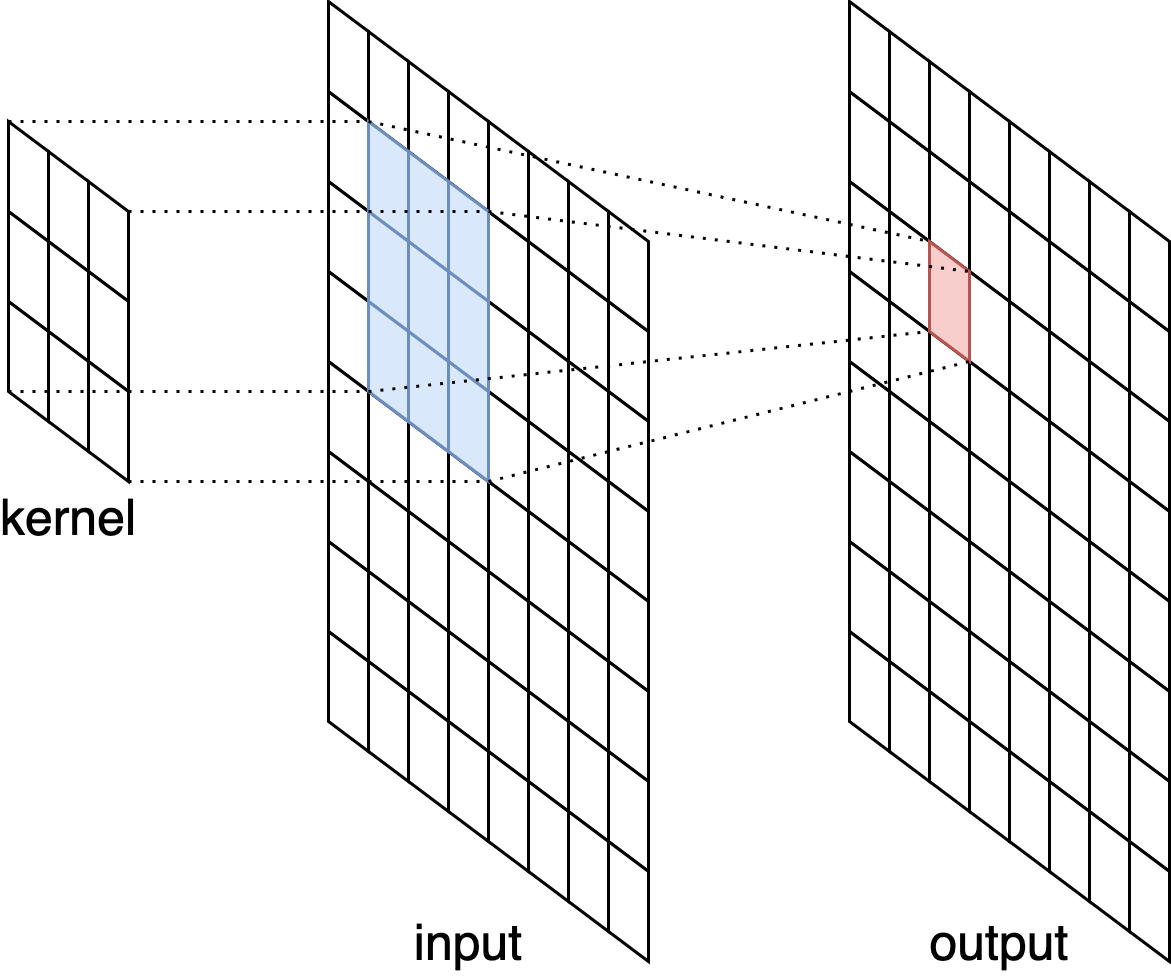
\includegraphics[width=0.4\linewidth]{images/Convolution}
	\caption{Convolutional Layer. The picture depicts a $3\times3$ kernal, that is convolved over a $5\times5$ image (input). Producing a $5\times5$ feature map (output).}
	\label{fig:Conv}
\end{figure}

This process of convolution can best be visualized as shining a flashlight over a dark image.\autoref{fig:Conv} As the flashlight moves (or `convolves') around the image,
it illuminates different parts, and the illuminated section is transformed through the filter. The output is a new image that highlights certain features—edges,
textures, or shapes—depending on what the filter is designed or has learned to detect.
The strength of convolutional layers is their ability to learn patterns with translational invariance. This means,
if a pattern is learned in one part of an image, the same pattern can be recognized in a different part without explicitly training for that location.
This property is especially advantageous for image recognition tasks where the same feature, such as the edge of an object or the texture of a surface, can appear anywhere in the image.

In summary, convolutional layers form the foundational building block of CNNs, enabling the network to automatically learn hierarchical and spatially invariant features,
which are essential for tasks like image classification, object detection, and many other applications in the realm of computer vision.

\subsection{UNet Architecture}
Building on the foundational principles of Convolutional Neural Networks,
the U-Net architecture presents a specialized deep learning structure that has proven to be highly effective for tasks like biomedical image segmentation.
Originally introduced by Olaf Ronneberger, Philipp Fischer, and Thomas Brox in 2015\cite{ronneberger_u-net_2015}, U-Net addresses challenges unique to medical imaging, such as the need for high-resolution output,
fewer training samples, and intricate structures.

\begin{figure}[!hb]
	\centering
	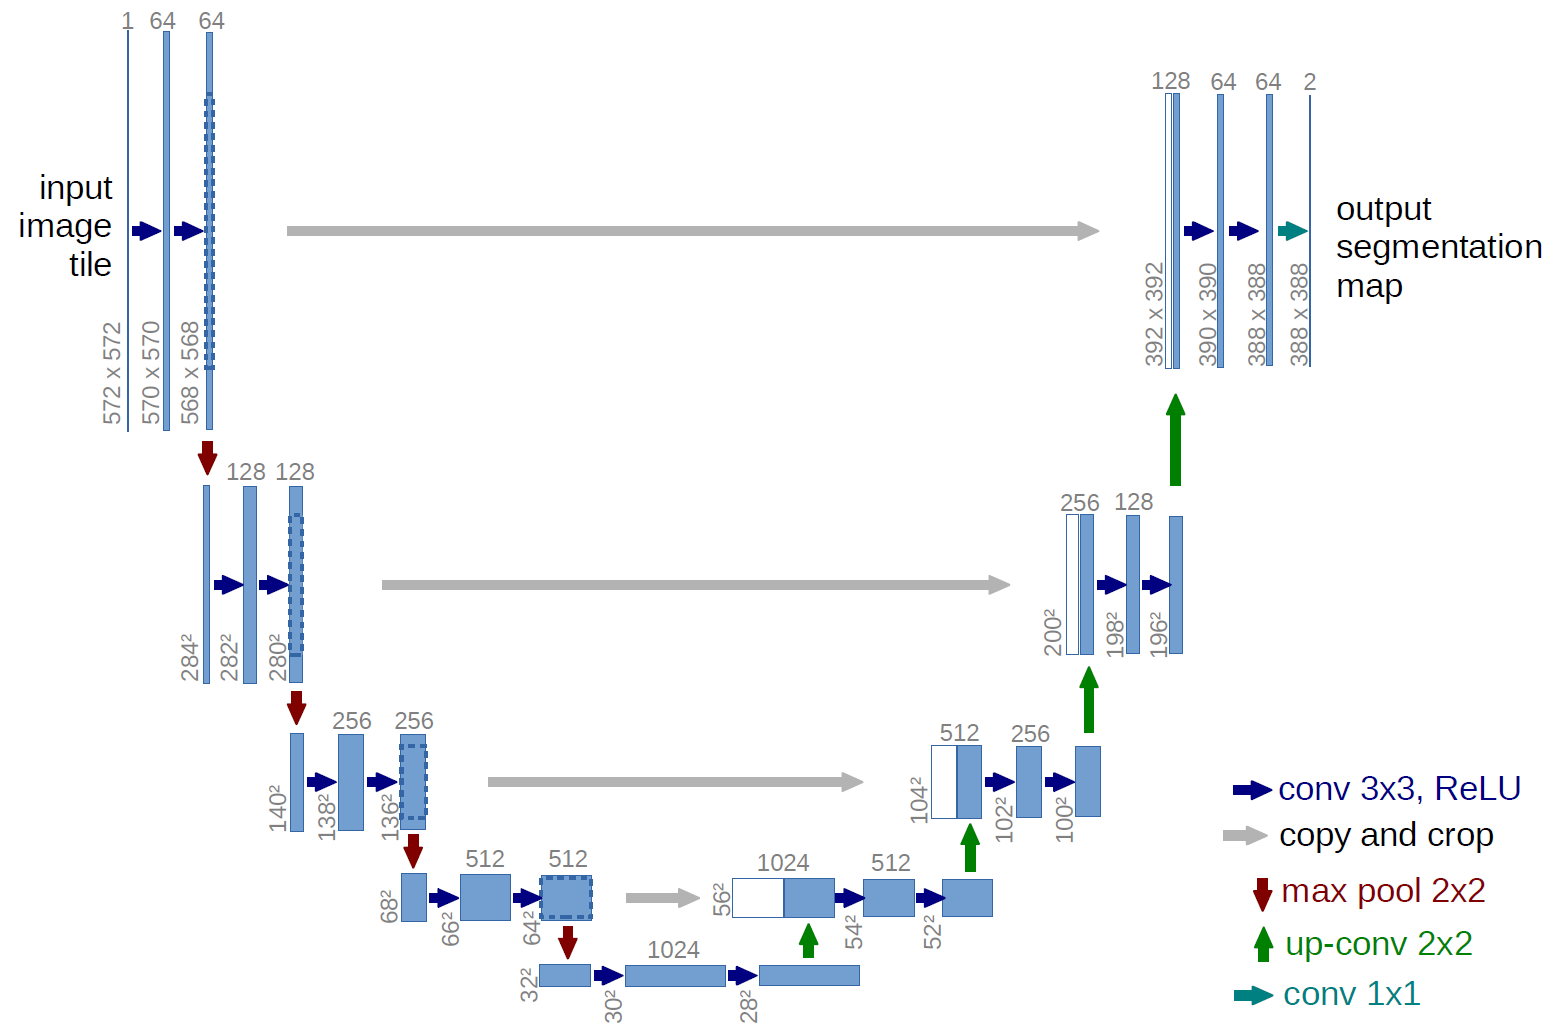
\includegraphics[width=0.8\linewidth]{images/UNet-Architecture}
	\caption{UNet Architecture. Each blue
	box corresponds to a multi-channel feature map. The number of channels is denoted
	on top of the box. The x-y-size is provided at the lower left edge of the box. White
	boxes represent copied feature maps. The arrows denote the different operations.\cite[2]{ronneberger_u-net_2015}}
	\label{fig:UNet}
\end{figure}

\noindent The name `U-Net' is derived from its U-shaped architecture.
This shape essentially consists of two primary parts:
\newpage
\noindent\textbf{Contracting (Downsampling) Path}\\
This is the `encoder' and looks very much like a traditional CNN.
Starting with the input image, this pathway consists of a series of convolutional layers followed by max-pooling layers.
As we move deeper into the network through this path,
the spatial dimensions of the feature maps decrease, but the depth (number of channels) increases.
This captures increasingly abstract representations of the input image,
compressing the spatial information but enriching the contextual details.

\noindent\textbf{Expansive (Upsampling) Path}\\
This is the `decoder' where the U-Net starts to differentiate itself from other CNNs.
In this path, the spatial dimensions of the feature maps are gradually increased using up-convolutions
(or transposed convolutions). This helps recover the spatial information required for precise segmentation.
Additionally, at every step of this pathway, there's a crucial skip connection from the corresponding layer in the contracting path.
This means that the high-resolution features from the downsampling path are concatenated with the upsampled features.
Such skip connections ensure that the localization information is not lost,
which is crucial for achieving precise boundaries in segmentation tasks.\cite[4]{ronneberger_u-net_2015}

\noindent The final layer of the U-Net is a convolution that maps the multi-channel feature map to the desired number of classes, essentially assigning each pixel of the image to a particular segment.\\

\noindent\textbf{Advantages and Challenges}\\
This intricate structure allows the UNet to capture high resolution local information in the upper parts of the UNet and low resolution global information in the bottom part to the UNet,
enabling it to come up with precise and accurate segmentations. The skip connections are particularly significant, bridging the gap between the high-resolution input and precise segmentation output.
Moreover, U-Net's efficient use of data, requiring fewer annotated images for training, is a significant advantage, especially in the domain of biomedical imaging where labeled data can be scarce.\\
However, every silver lining has its cloud. One of the challenges when using the U-Net architecture arises when handling high-resolution 3D data. While U-Net excels with high-resolution 2D images,
translating this to 3D data dramatically increases the computational and memory demands. This is primarily due to the increase in spatial dimensions: in 3D,
every slice of data contributes additional information that the network must process, making the memory footprint substantially larger. As a result,
processing large 3D datasets can become particularly taxing on the GPU memory. This limitation can make the architecture unsuitable for consumer-grade graphics cards,
hindering its widespread application in some 3D imaging contexts.
\newpage
\subsection{Patch-wise UNet}
Given the inherent challenges posed by the U-Net architecture when managing high-resolution 3D datasets, there emerges an essential need to develop a more adaptable and resource-efficient approach.
Enter the patch-wise UNet.\\
The patch-wise UNet operates on the principle of segmenting the larger 3D dataset into smaller, manageable patches, allowing for individual processing of each segment.
This methodology dramatically reduces the GPU memory demands. However, with every solution comes its unique set of challenges.
By segmenting the dataset and analyzing it in patches, the neural network inherently loses the global context of the entire image.
This local view can potentially compromise the accuracy of segmentations as the model might miss out on leveraging crucial information from neighboring patches.
In essence, while the patch-wise UNet offers a solution to memory constraints, it introduces the trade-off of potentially reduced accuracy due to the loss of global information.

\subsection{UNet Cascade}
Independent of memory efficency the UNet cascade proposed in the nnUNet paper\cite{isensee_nnu-net_2018} trys to improve the capabilitys of the UNet to
segment fine structures by using a two stage approach.

\begin{figure}[!hb]
	\centering
	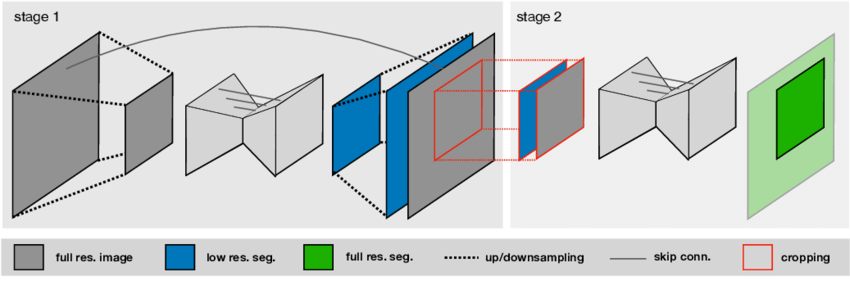
\includegraphics[width=1\linewidth]{images/UNet-Cascade}
	\caption{UNet-Cascade\cite{simpson_large_2019}}
	\label{fig:UNet-Cascade}
\end{figure}

\noindent\textbf{Stage 1:}\\
The process begins by downsampling the input images to a lower resolution. This reduction simplifies the image while retaining its core structural elements.
A standard U-Net then processes this low-resolution image, producing a segmentation that primarily captures the broader, global features.
While some detail is inevitably lost due to the reduced resolution,
this stage effectively provides an initial segmentation that identifies the general areas of interest within the scan.

\noindent\textbf{Stage 2:}\\
The low-resolution segmentation from the first stage is then upscaled back to the original image size. This upscaled segmentation, capturing broad structures,
is concatenated with the original high-resolution scan, creating a guided version of the scan.
By merging the global information from the upscaled segmentation with the local detail of the original scan, a richer context is formed.
This guided scan is then cropped to focus on areas where the first stage identified potential regions of interest.
A standard UNet then processes this cropped, guided scan, refining the segmentation further, honing in on the finer structures with greater precision.

The U-Net cascade, in its essence, is a solution that seeks to balance the global and local context.
By starting with a bird's-eye view and then refining with granular detail,
it aims to produce segmentations that capture intricate structures more accurately than a single-stage U-Net might.

To address memory constraints, especially in situations with limited computational resources, this two-stage structure can be adapted. Specifically,
the second stage can be modified to operate on sliced patches.
While this approach would inherently trade off some accuracy due to the loss of broader context outside each patch,
it offers a way to make the cascade more memory-efficient while still benefiting from the two-stage refinement process.
This modified cascade is the main focus of our investigation.

\chapter{Methodology}
In this work, we focused on a competitive analysis of various medical segmentation models with the objective of assessing the tradeoffs between performance, inference time and memory efficiency.
For the models we focus on different variations of the UNet architecture. The models employed for the training and evaluation include the use of normal 3D UNet, patch-wise UNet,
patch-wise UNet cascade. For a compatitive analysis we implemented them in PyTorch and trained them on the Medical Segmentation Decathlon (MSD) datasets.\\

\section{Data Collection and Preparation}
The first section of the methodology revolves around the selection and conditioning of datasets employed in model training and evaluation.
Recognizing the disparities among Medical Image Segmentation tasks, we aimed for a broad evaluation by training our models on diverse datasets.
The Medical Segmentation Decathlon (MSD) offers ten distinct, task-specific datasets, witch can be downloaded from http://medicaldecathlon.com/.
All the data was made available under the Creative Commons license CC-BY-SA 4.0. This license allows us to use the data by citing this paper.\cite{simpson_large_2019}

\begin{table}[ht!]
\begin{center} {\footnotesize
\begin{tabular}{lccc}
\hline
	& \multicolumn{3}{c}{MSD Dataset}  \\
	& \multicolumn{1}{c}{size} & \multicolumn{1}{c}{shape} & \multicolumn{1}{c}{mean voxel count}\\
\hline
Task01\_BrainTumor & $484$ & $240\times240\times155$ & $8.928.000$ \\[1ex]
Task02\_Heart & $20$ & $320\times320\times90\mbox{-}130$ & $11.627.520$ \\[1ex]
Task03\_Liver & $131$ & $512\times512\times74\mbox{-}987$ & $117.340.457$ \\[1ex]
Task04\_Hippocampus & $260$ & $31\mbox{-}43\times40\mbox{-}59\times24\mbox{-}47$ & $62.793$ \\[1ex]
Task05\_Prostate & $32$ & $256\mbox{-}384\times256\mbox{-}384\times16\mbox{-}24$ & $1.924.224$ \\[1ex]
Task06\_Lung & $63$ & $512\times512\times112\mbox{-}636$ & $73.471.057$ \\[1ex]
Task07\_Pancreas & $281$ & $512\times512\times37\mbox{-}751$ & $24.926.070$ \\[1ex]
Task08\_HepaticVessel & $303$ & $512\times512\times24\mbox{-}181$ & $18.272.215$ \\[1ex]
Task09\_Spleen & $131$ & $512\times512\times31\mbox{-}168$ & $23.337.210$ \\[1ex]
Task10\_Colon & $126$ & $512\times512\times37\mbox{-}729$ & $28.057.730$ \\[1ex]
\hline
\end{tabular} }
\end{center}
\caption{\footnotesize This table shows the size, shape and mean voxel count of eatch MSD datasets.
The shape is given as $\text{width}\times \text{height}\times \text{depth}$ when a dimention is variable it is given as $\text{min}\mbox{-}\text{max}$.
Thee mean voxel count is calculated by taking the mean of the product of the width, height and depth and then taking the mean rounding down to the next intager.}
\label{turns}
\end{table}
\noindent While memory efficiency is a problem on images with large voxel count it is not so prominent for images with a low voxel count.
As our emphasis lay on addressing memory efficiency challenges associated with large voxel counts, we did not choose datasets with a low voxel count.
Since brain tumor segmentation is the most common dataset for medical image segmentation research we chose the Brain Tumor dataset as our primary dataset.
To test the capabilitys on datasets with a larger voxel count we chose the Liver dataset as our secondary dataset.\\

\noindent In the final stage of preparation, all image data undergo normalization, and both images and labels are converted into 4D Tensors, adhering to the shape (channel, width, height, depth).
Notably, no form of data augmentation is applied. To ensure a rigorous model evaluation, we partition the datasets into three distinct subsets: training, validation, and testing.
The training subset is used for the training of the model, the validation subset assesses accuracy during this training phase, while the testing subset is reserved for the ultimate model evaluation.
Specifically, the datasets is split as follows: 60\% for training, 20\% for validation, and 20\% for testing.

\section{Model Description}
Our investigation covers the following models: standard 3D UNet, patch-wise 3D UNet, and patch-wise 3D UNet cascade.

\subsection{3D UNet}
Our choice of a foundational model is the standard 3D U-Net, which has proven its prowess in a range of segmentation tasks.
At its inception, the model commences with a convolutional layer designed to generate 32 channels. As data progresses deeper into the network,
these channels expand in number, marking the distinct stages of the descending U-Net structure with output channels scaling at 64, 128, 256, and finally culminating at 512.

While the quintessential U-Net relies on double convolutions at each of its stages, we sought improvements in this domain. To achieve this,
every stage in our U-Net is composed of two sequential convolution layers. Each convolution layer, characterized by a kernel size of 3 and a padding of 1,
is immediately followed by a Batch Normalization (BatchNorm) layer with a momentum of 0.1 and a Rectified Linear Unit (ReLU) activation function.\cite{ioffe_batch_2015}
This modified architecture ensures more efficient training and potentially better generalization. The final output is then passed throu a softmax activation function.

Despite the advancements and the precision it offers, our 3D U-Net reveals its Achilles heel when confronted with datasets boasting a hefty voxel count.
Its memory consumption makes it a formidable contender for standard GPUs, necessitating the use of high-tier graphics cards like the A40 or A100 to process such extensive datasets efficiently.

\subsection{patch-wise UNet}
Prioritizing GPU memory efficiency, the patch-wise UNets present a viable alternative. It maintains specifications consistent with the 3D UNet.
The patch-wise UNet slices the input is size 16 patches then segments them indeviualy. In instances where image dimensions aren't multiples of 16, the final patch undergoes zero-padding.
The preduced patch segmentations are then reconstructed to a full segmentation.
These adaptations considerably diminish GPU memory consumption but also tend to compromise on accuracy because of the loss of global context.

\subsection{patch-wise UNet cascade}
In contrast to the previously discussed UNets that produce segmentations at full resolution, the cascade approach follows a two-stage process:
initial segmentation at a reduced resolution, followed by a refinement at full resolution.\\
\textbf{Stage 1:}
The input images are downscaled by a factor of 0.3 for BrainTumor and a factor of 0.2 for the Liver dataset, producing a image with reduced resolution. These downscaled images are then processed through a 3D UNet,
yielding a low-resolution segmentation.
\textbf{Stage 2:}
The segmentation from the first stage is upscaled back to its original size and acts as guidance for the subsequent stage.
This upscaled segmentation is concatenated with the original image and then passed in to a patch-wise UNet in the second stage with se same specifications as the normal patch-wise UNet.\\

\noindent The key advantage of this cascade structure is memory efficiency. Both the patch-wise and the 3D UNet operating on downscaled images inherently require less memory.
This makes the cascade method more memory-efficient compared to the standard 3D UNet that operates at full resolution. Furthermore,
the low-resolution segmentation from the first stage is designed to compensate for the loss of spatial information, potentially enhancing the accuracy of the segmentation in the second stage.
As a result, the cascade UNet is anticipated to deliver more accurate results than the standalone patch-wise UNets.

\section{Environment and Tools}
All model training and evaluations were conducted using an NVIDIA A40 GPU with 48GB of GPU memory. The experiments operated under a Linux Ubuntu 20.04 amd64 environment. For the model's implementation,
we utilized the PyTorch framework.

\section{Training}
As the training process is a crucial component of our investigation, we elaborate on the training methodology in this section.
\subsection{Loss Function}
We employ Dice Loss for training the UNets. Witch is given by this formula where TP is the number of true positives, FN is the number of false negatives and FP is the number of false positives.
$$\mathcal{L}_{dice}=\frac{2*\text{TP}}{2*\text{TP}+\text{FN}+\text{FP}}$$
Given that our segmentations invariably incorporate a background channel, this channel is excluded from consideration.
The rationale behind this is that many images predominantly consist of background, and inclusion of this background could disproportionately dominate the loss calculation.
A potential pitfall emerges when the ground truth segmentation comprises solely of the background. In such instances, the model only generates true negatives and false positives,
leading to a consistent Dice Loss value, rendering gradient computation impossible. However, when training on entire images,
this issue is circumvented as all images contain non-background segmentations. Conversely, for the patch-wise UNet, where only sections of images serve as training data,
instances may arise where the ground truth segmentation consists only of the background. To address this,
we ensure that the background channel is incorporated into the loss calculation for the patch-wise UNet.

\subsection{Optimizer}
Across all experiments, we employ Adaptive Momentum Estimation (Adam)\cite{kingma_adam_2017} as our optimizer.
Instead of having a constant learing rate Adam adjusts the learning rate at each iteration based on momentum, proving efficient in practice. For initialization,
a learning rate of 3e-4 is set. This uniform choice of learning rate across experiments aids in comparability, ensuring that the learning rate parameter does not significantly skew accuracy results.

\subsection{Epochs and Steps}
Since the datasets all very in size, we choose a constant step count instead of a constant epoch count. All models are trained on 100.000 steps.
We made checkpoints after each epoch and chose the checkpoint with the best validation accuracy as the final model.

\section{Evaluation Metrics}
Upon completion of the training phase, the models are evaluated based on three pivotal metrics: accuracy, inference time, and GPU memory consumption during inference.
Each model is subject to inference on the test datasets 40 times, and the arithmetic mean for each metric is then computed.

\subsection{Accuracy}
We gauge accuracy by computing the Dice Loss on the complete segmentations. Given that none of the segmentations is solely composed of background, we exclude the background channel in our calculations,
as elaborated in section 3.4.1. For slice/patch-wise segmentation the accuracy is computed on the reconstructed segmentation and not on the individual slices/patches.

\subsection{GPU Memory Monitoring}
To determine GPU memory efficiency, we record the GPU memory allocation immediately post-inference, when both the model and data persist on the GPU.
For the cascade this is done once after stage one and once after stage two. This metric is anticipated to maintain a consistent reading throughout the evaluation phase.

\subsection{Inference Time}
An accurate representation of model efficacy also mandates the measurement of inference time – the duration a model requires to annotate a single image.
The stopwatch is activated the moment an image is fed into the model and halted once the output is generated. For slice/patch-wise models,
the metric encapsulates the time consumed to segment the entirety of the image.

\chapter{Implementation}
Our project primarily utilizes the PyTorch framework due to its flexibility and widespread adoption in the deep learning community.
\section{Model}
Our foundational architecture was the 3D U-Net. Interestingly, a single class was developed to represent all three U-Net variations. The uniqueness of each U-Net type emerged not in the architectural structure,
but rather in their distinct training and inference methodologies.
\section{Dataset Loading with MSDDataset}
To streamline data handling, the MSDDataset class was established. This class serves the pivotal role of loading and preprocessing the Medical Segmentation Decathlon (MSD) datasets.
One of its primary functions is to interpret the dataset.json file inherent to every MSD dataset. This JSON file delineates dataset attributes such as its type, the significance of input and output channels,
and the directory paths to the respective images and labels. Upon these directives, the MSDDataset class proceeds to load, normalize, and prepare the datasets for subsequent stages.\\
To facilitate diverse data transformation requirements, we introduced a suite of wrapper datasets:
\begin{enumerate}
	\item DownsampledDataset: Engages the PyTorch's Upsample class to downscale both images and labels. An inherent rescaling function allows it to restore the datasets to their native resolutions when needed.
	\item SlicedDataset: This dataset wrapper slices the image and label in to patches of the same size, padding the last patch of needed.
	A reconstruction function is embedded for scenarios necessitating a revert to the original dataset dimensions.
	\item CombinedDataset: This is a hybrid class that amalgamates two datasets. While it offers customizable combination functions,
	its default behavior is to concatenate the first dataset's image with the second dataset's label, thereby formulating a new image-label pair.
\end{enumerate}

\section{Training Framework}
For the training we implemented four trainer classes. Eatch training setup uses data loaders for efficient asynchronous data loading.
The type of dataset and model requirements dictate our choice of data loader and associated wrappers. Here's a breakdown:

\begin{enumerate}
	\item 3D UNet: For the standard 3D U-Net, we mainly use the MSDDataset class. It allows us to go through the entire dataset, one epoch at a time.
	\item Patch-wise 3D U-Net: For this version, we use the MSDDataset class wrapped within the SlicedDataset. This setup divides the data into patches.
	In each step backpropagation is done on all patches of the current image.
	\item Patch-wise 3D U-Net Cascade: The first stage is trained using the MSDDataset class inside the DownSampleDataset wrapper. This wrapper initially downscales the dataset to fit the requirements of this stage.
	The process for this stage involves several steps:
	\begin{enumerate}
		\item Start with wrapping the MSDDataset in the DownSampleDataset wrapper, set to downscale and then rescale the image and label.
		\item Next, the CombinedDataset wrapper merges the rescaled label with the original image, providing the new input. The original label is kept as the ground truth.
		\item This combined dataset is then wrapped with the SlicedDataset to train the model on patches, similar to the patch-wise U-Net approach.
	\end{enumerate}
\end{enumerate}

The model's training can be started using a dedicated script that accepts configuration files as input. These files are amalgamated into a comprehensive configuration dictionary,
which in turn drives the initialization of the apt training class.\\[1ex]
\section{Model Evaluation}
The model can be evaluated using three differen evaluator classes. Eatch evaluator class uses a data loader to load the data.
For the cascade the two stage are conected together to evaluate the performance of the entire cascade. Every results during training and evaluation are logged using Weights and Biasis.

\chapter{Experimental Results}

In our journey to improve and adapt the U-Net architecture, it's crucial to see how well our changes work in practice. In this chapter,
we present the results garnered from our experiments, which provide a clear picture of the advantages, trade-offs, and potential areas of improvement associated with our implementations.
The first Dataset we trained our models on was the Brain Tumor dataset.

\begin{table}[ht!]
\begin{center} {\footnotesize
\begin{tabular}{lccc}
\hline
	& \multicolumn{3}{c}{Brain Tumor Dataset accuracy} \\
	& \multicolumn{1}{c}{edema} & \multicolumn{1}{c}{non-enhancing tumor} & \multicolumn{1}{c}{enhancing tumor}\\
\hline
3D UNet & $\mathbf{80.13}$ & $\mathbf{60.80}$ & $\mathbf{75.99}$ \\[1ex]
patch-wise UNet & $70.01$ & $31.02$ & $55.58$ \\[1ex]
patch-wise UNet cascade & $77.54$ & $56.84$ & $71.18$ \\[1ex]
\hline
\end{tabular} }
\end{center}
\caption{\footnotesize This table shows the mean dice scores for the Test split of the Brain Tumor dataset. The best scores are highlighted in bold.}
\label{turns}
\end{table}

\noindent The 3D UNet demonstrates superior performance in all metrics. While the patch-wise UNet has the least impressive results across categories,
the patch-wise UNet cascade fares better. Notably, it surpasses the patch-wise UNet considerably and even approaches the 3D UNet's precision.
Inspecting the results we notice that all models struggle to segment more fine structures like the non-enhancing tumor.\\

\begin{table}[ht!]
\begin{center} {\footnotesize
\begin{tabular}{lccc}
\hline
	& \multicolumn{2}{c}{Brain Tumor Dataset efficiency} \\
	& \multicolumn{1}{c}{GPU memory(GB)} & \multicolumn{1}{c}{inference time(s)} \\
\hline
3D UNet & $21.5$ & $\mathbf{0.35}$ \\[1ex]
patch-wise UNet & $2.9$ & $0.67$ \\[1ex]
patch-wise UNet cascade & $\mathbf{2.8}$ & $0.91$\\[1ex]
\hline
\end{tabular} }
\end{center}
\caption{\footnotesize This table shows the mean inference time for the Test split of the Brain Tumor dataset over 30 epochs in seconds and the max GPU memory consumption in GB.
The best scores are highlighted in bold.}
\label{turns}
\end{table}

The standard 3D UNet is the most demanding in terms of GPU memory. Intriguingly, the patch-wise UNet cascade consumes less memory than its standard counterpart,
even though it inherently incorporates the patch-wise UNet. In terms of inference time, the 3D UNet shines the brightest, whereas the cascade model lags behind the standard patch-wise model probably due to its two-stage processing.\\[1ex]
Let us now take a look at the results for Liver dataset.

\begin{table}[ht!]
\begin{center} {\footnotesize
\begin{tabular}{lccc}
\hline
	& \multicolumn{2}{c}{Liver Dataset accuracy} \\
	& \multicolumn{1}{c}{liver} & \multicolumn{1}{c}{cancer} \\
\hline
3D UNet & $-$ & $-$ \\[1ex]
patch-wise UNet & $87.01$ & $22.22$ \\[1ex]
patch-wise UNet cascade & $\mathbf{92.00}$ & $\mathbf{25.05}$ \\[1ex]
\hline
\end{tabular} }
\end{center}
\caption{\footnotesize This table shows the mean dice scores for the Test split of the Liver dataset. The best scores are highlighted in bold.}
\label{turns}
\end{table}

The patch-wise UNet cascade claims the top spot for performance on the Liver dataset. The 3D UNet, on the other hand, was not able to produce any results doe to the extensive voxel count.
When focusing on segmenting cancer, the models showed room for improvement. However, liver segmentation showed promising results.

\begin{table}[ht!]
\begin{center} {\footnotesize
\begin{tabular}{lccc}
\hline
	& \multicolumn{2}{c}{Liver Dataset efficiency} \\
	& \multicolumn{1}{c}{GPU memory(GB)} & \multicolumn{1}{c}{inference time(s)} \\
\hline
3D UNet & $\geq325$ & $-$ \\[1ex]
patch-wise UNet & $\mathbf{10.6}$ & $\mathbf{4.49}$ \\[1ex]
patch-wise UNet cascade & $12.4$ & $5.90$\\[1ex]
\hline
\end{tabular} }
\end{center}
\caption{\footnotesize This table shows the mean inference time for the Test split of the Liver dataset over 30 epochs in seconds and the max GPU memory consumption in GB. The best scores are highlighted in bold.}
\label{turns}
\end{table}

When it comes to the Liver dataset we encountered some problems. The 3D UNet was not able to train on the Liver dataset due to the large voxel count.
The training process would run out of memory when the model tryed to allocate 325 GB of GPU memory.
The patch-wise UNet, though trainable, initially produced only background segmentations.
We pinpointed the inclusion of the background channel in the loss calculation as the culprit. By excluding this channel,
the model's training performance improved significantly. Given the 3D UNet's memory requirements,
this model isn't a feasible choice even for high-end GPUs like the A100. Implementing it across multiple GPUs might be a solution, but it brings its own set of challenges.
Conversely, both patch-wise models prove to be adaptable choices for conventional GPUs with 16 GB or more memory.

\chapter{Discussion}
In this section, we dive into the implications of our experimental findings, addressing both the strengths and constraints of our study, along with potential avenues for further refinement.\\
Our results from the Brain Tumor dataset indicate that the 3D UNet stands out in terms of accuracy. However, this prowess is accompanied by increased GPU memory demands.
This isn't an issue for datasets with moderate voxel counts, such as the Brain Tumor dataset, but it emerges as a constraint for voluminous datasets like the Liver dataset.\\
Assuming the GPU memory consumption scales linearly with voxel count (a plausible assumption given the linear scaling of all convolutional layers),
an average scan from the liver dataset would necessitate a memory allocation of approximately $\frac{21,5~\text{GB} * 117.340.457}{8.928.000}\approx282~\text{GB}$.
For the inaugural Liver dataset scan, which was halted because of an attempted 325 GB allocation, the scan's size was $512\times512\times771$,
resulting in an estimated memory demand of $\frac{21,5~\text{GB} * 512*512*771}{8.928.000}\approx486~\text{GB}$. This far exceeds the capacity of a single GPU.
To illustrate, NVIDIA's A100 offers a peak memory of $100~\text{GB}$, and even this premium GPU falls short. Addressing this would necessitate employing multiple GPUs,
bringing the added complexity of multi-GPU support.\\
Our findings posit the patch-wise UNet and its cascade counterpart as promising alternatives.
Notably, the cascade variant has longer infernece time then the normal patch-wise UNet and is more complex to train since one has to tain two networks. However,
this cascade structure elevates the accuracy of the model by far, making it compatible to the normal UNet. When pitted against the cascade,
the sole advantages of the standard patch-wise UNet are its swifter inference times and simpler implementation. Given these trade-offs,
we advocate for the patch-wise UNet cascade over its simpler counterpart in most scenarios.\\
For datasets comprising low-resolution images, the original 3D UNet remains the gold standard due to its superior speed and accuracy.
Yet, when tackling high-resolution imagery, the patch-wise UNet cascade emerges as a worthy contender.\\
While our models have demonstrated potential, there remains a significant gap between our results and the benchmarks set by contemporary studies.
For context, in the nnUNet paper, competitors of the MSD achieved a dice score of $73.71$ for cancer detection in the Liver dataset.
When juxtaposed with our dice score of $25.05$ for the same task, the disparity is evident: our models are not yet on par with the best in the field.
Several strategies could bridge this gap:
\begin{enumerate}
	\item \textbf{Data Augmentation}: Introducing variations in the training data through techniques like rotation, scaling, and flipping can make our model more robust and potentially improve its generalization capability.
	\item \textbf{Focusing on the Region of Interest}: In the preprocessing phase, cropping images to highlight the region of interest can ensure the model's training focuses more intently on the salient data, potentially improving accuracy.
	\item \textbf{Leveraging Pre-training}: Training our model on diverse datasets before fine-tuning it on the specific dataset of interest can provide a more generalized feature representation,
	which might boost performance when the model is subsequently fine-tuned. Unsupervised learning techniques could also be employed to generate a more robust feature representation.
\end{enumerate}
By integrating these strategies, we belive to be able to enhance our model's performance and bring it closer to the state-of-the-art benchmarks in future iterations.
Other interesting further investigations could be to compare the patch-wise UNet cascade to outher models that try to address the memory efficiency problem. One outher woerthy contestent could be a memory efficient alternative to the 3D UNet,
is the Patch-free Segmentation model proposed in this paper\cite{wang_super-resolution_2023}.